\documentclass[a4paper,12pt]{article}

\usepackage[utf8]{inputenc}
\usepackage[T1]{fontenc}
\usepackage{a4}
\usepackage{lipsum}
\usepackage{graphicx}
\usepackage{float}
\usepackage{listings}
\usepackage{color}
\usepackage{hyperref}
\usepackage{cite}
\usepackage{textgreek}
\usepackage{amsfonts}

\usepackage[margin=1in]{geometry}

\definecolor{dkgreen}{rgb}{0,0.6,0}
\definecolor{gray}{rgb}{0.5,0.5,0.5}
\definecolor{mauve}{rgb}{0.58,0,0.82}

\lstset{frame=tb,
  language=matlab,
  aboveskip=5mm,
  belowskip=5mm,
  showstringspaces=false,
  columns=flexible,
  basicstyle={\small\ttfamily},
  numberstyle=\tiny\color{gray},
  keywordstyle=\color{blue},
  commentstyle=\color{dkgreen},
  stringstyle=\color{mauve},
  breaklines=true,
  breakatwhitespace=true,
  tabsize=2
}

\title{
  {\Huge \bf Power Systems Lab}\\
  \vspace{0.25in}

  {\bf Experiment 7}\\
  Laboratory Report
  \vspace{1in}
}
\author{
  \bf Syed Alisamar Husain, 17BEE012\\
  B.Tech Electrical Engg, 8th Semester
}

\begin{document}
  \begin{titlepage}
    \maketitle
    \vspace*{\fill}
    \begin{center}
      {\bfseries Department of Electrical Engineering} \\
      Jamia Millia Islamia, New Delhi
    \end{center}
    \thispagestyle{empty}
  \end{titlepage}
  
  \newpage
  \begin{center}
    \huge Experiment 7
    \vspace{0.5in}
  \end{center}

  \section{Objective}
  To verify the superposition theorem for a 3-phase radial 
  electrical power system using Simulink Simscape Electrical.

  \section{Theoretical Background}
  {\bf The Superposition Theorem states that a linear circuit can be analyzed with 
  only one source of power at a time,} the corresponding component voltages and currents 
  algebraically added to find the net effect of all power sources.\\
  
  To negate all but one power source for analysis, replace any source of voltage 
  (batteries) with a wire; replace any current source with an open (break).

  It must be noted, that the Superposition Theorem works only for circuits 
  that are reducible to series/parallel combinations for each of the power sources 
  at a time. Thus, this theorem can't be used for analyzing an unbalanced bridge 
  circuit, and it only works where the underlying equations are linear (no 
  mathematical powers or roots). 

    \subsection{Prerequisites for Applicablility}
    The requisite of linearity means that Superposition Theorem is only applicable 
    for determining voltage and current, not power. Power dissipations, being 
    nonlinear functions, do not algebraically add to an accurate total when only 
    one source is considered at a time. The need for linearity also means this 
    Theorem cannot be applied in circuits where the resistance of a component 
    changes with voltage or current. Hence, networks containing components like 
    lamps (incandescent or gas-discharge) or varistors could not be analyzed.

    Another prerequisite for Superposition Theorem is that all components must be 
    {\bf bilateral}, meaning that they behave the same with electrons flowing in either 
    direction through them. Resistors, inductors and capacitors being studied must 
    have no polarity-specific behavior.

    The Superposition Theorem finds use in the study of alternating current (AC) 
    circuits, and semiconductor (amplifier) circuits, where sometimes AC is often 
    mixed (superimposed) with DC. Because AC voltage and current equations (Ohm’s Law) 
    are linear just like DC, we can use Superposition to analyze the circuit with 
    just the DC power source, then just the AC power source, combining the results 
    to tell what will happen with both AC and DC sources in effect.

  \pagebreak
  \section{Implementation}
  For the verification of the superposition theorem, we build a model to represent
  the three phases of a 3-phase power system, each 120 degrees apart.
  Each phase has an independent voltage source and a {\bf line resistance} in series 
  with a {\bf load impedance.} These resistances and impedances are equal for every
  phase, thus making the system balanced.
  \begin{figure}[H]
    \centering
    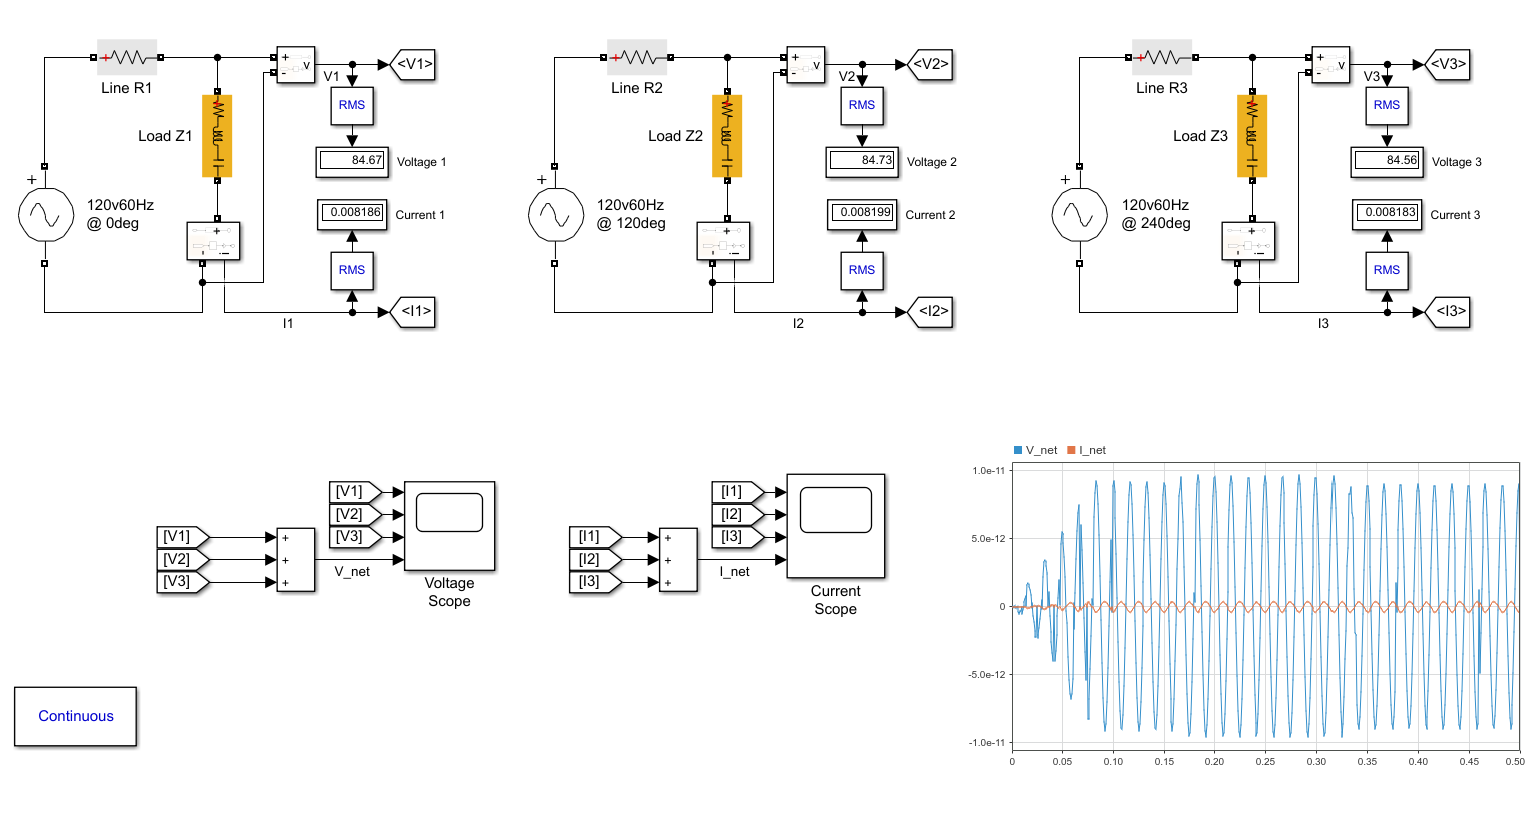
\includegraphics[width=6in]{img/model.png}
  \end{figure}

  \section{Observations}
  We measure the sum of voltages and currents which will give us the voltage at the
  null-point of a Y-connected load. For a three-phase system we expect that {\bf the sum
  of currents at the null point should be zero}, since the sum of three sine waves
  120 degrees out of phase with each other is zero at every point.

  \begin{figure}[H]
    \centering
    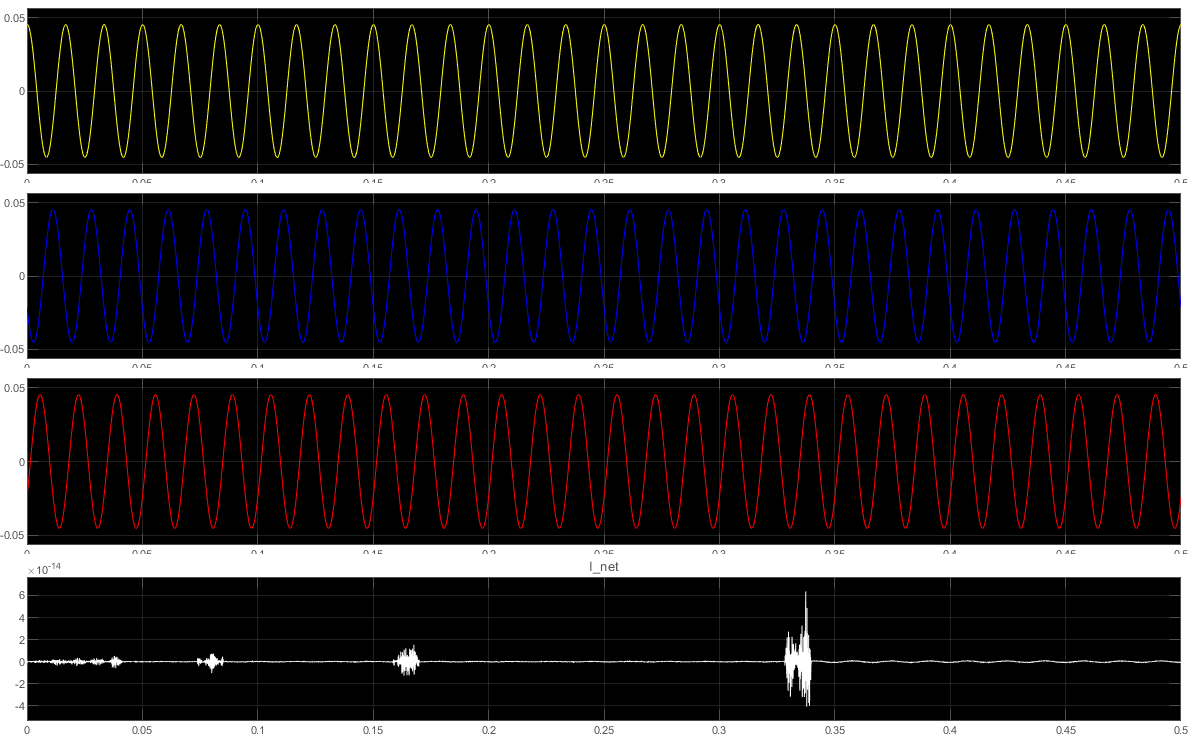
\includegraphics[width=4.5in]{img/I_scope.png}
  \end{figure}
  \pagebreak
  From the graph we can see that the currents at the null-point sum to zero, thus
  proving that the sum of currents of three independent phases is the same as the 
  current of a 3-phase system. This means that each voltage source can be considered
  independently, {\bf hence proving the superposition theorem.}

  \section{Result}
  We proved and verified that superposition theorem for a 3-phase power system using
  a Simulink model.

\end{document}